\documentclass[aps,pra,reprint,superscriptaddress,nofootinbib,longbibliography,floatfix]{revtex4-2}

% Keep otherwise identical pdfTeX builds byte reproducible.
\ifdefined\pdfinfoomitdate\pdfinfoomitdate=1\fi
\ifdefined\pdftrailerid\pdftrailerid{}\fi
\ifdefined\pdfsuppressptexinfo\pdfsuppressptexinfo=-1\fi

\usepackage{amsmath,amssymb,graphicx,microtype,placeins}
\usepackage{xcolor}
\definecolor{linkblue}{HTML}{1F4E79}
\usepackage[
  colorlinks=true,
  linkcolor=linkblue,
  citecolor=linkblue,
  urlcolor=linkblue
]{hyperref}
\hypersetup{
  pdftitle={When Can Reset-Window QELMs Emulate the Input--Output Behavior of Quantum Reservoirs?},
  pdfauthor={Anonymous Authors}
}

\graphicspath{{../figures/information_interface/}{../figures/compact_pra/}{../figures/canonical_emulation/}{../../pra_extension/figures_pra_final_v6/}}
\newcommand{\QRC}{\mathrm{QRC}}
\newcommand{\QELM}{\mathrm{QELM}}
\newcommand{\nrmse}{\mathrm{NRMSE}}
\newcommand{\risk}{\mathcal R}
\newcommand{\hist}{H_d}

\begin{document}

\title{When Can Reset-Window QELMs Emulate the Input--Output Behavior of Quantum Reservoirs?}
\author{Anonymous Authors}
\noaffiliation
\date{1 September 2026}

\begin{abstract}
A quantum extreme learning machine (QELM) transforms inputs into quantum
features for a trainable readout without carrying memory between predictions.
Encoding a window of recent inputs allows it to process temporal information.
Can such a window QELM reproduce a quantum reservoir computer (QRC), which
carries information between inputs in a quantum state?
We characterize when this replacement is possible. Two histories with
identical recent inputs are indistinguishable to a window model, yet may
produce different reservoir outputs. For scalar outputs, half the largest
such difference is exactly the smallest achievable worst-case error. Under
suitable regularity assumptions, a growing universal QELM family evaluated
through exact expectations can approach this optimum at every window length.
Arbitrary accuracy is therefore possible precisely when the difference
vanishes uniformly as the window grows. Only
memory that can affect the chosen outputs must fade. The full quantum state
need not forget its past. A two-qubit example demonstrates persistent memory
that prevents arbitrarily accurate finite-window replacement. Simulations
examine the practical roles of window length, feature capacity, and
measurement budgets. Together, these results establish when explicitly
encoded input history can replace recurrent quantum memory and when
information beyond any finite window remains essential.

\end{abstract}

\maketitle

\section{Introduction}
\label{sec:introduction}

Temporal models can use the past in two ways.  A recurrent model carries an
internal state from one input to the next.  A window model instead receives
recent inputs explicitly and starts each prediction afresh.  These choices
can describe the same input--output behavior, but only if the window contains
the information that still matters to the output.

\begin{figure*}[t]
 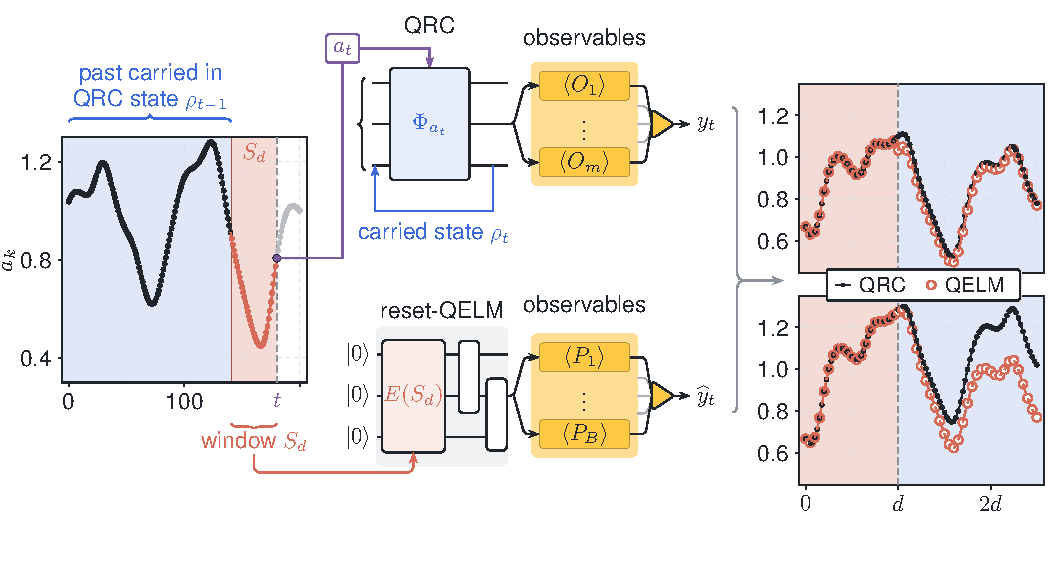
\includegraphics[width=\textwidth]{fig01_information_interface.pdf}
\caption{\textbf{When can finite context replace recurrent quantum memory?}
 \textbf{a} The QRC carries state; the reset-QELM receives the bracketed green window.
 Violet marks current input; grey continuation is excluded.
 Both have model-specific observables and trainable readouts; the target readout stays fixed during emulation.
 Right: the QRC retains an input after it leaves the window. The ideal window predictor
 cannot distinguish its two possible values; green shows their output midpoint for
 one history, not measured QELM performance.
 \textbf{b} For scalar outputs, $D_d/2$ is the smallest worst-case absolute error of
 any window predictor; $D_d$ is the largest output gap between histories sharing
 their last $d$ inputs but differing earlier. Longer windows can reach $\varepsilon$
 unless a higher floor persists. The output example and panel b are schematic.}
 \label{fig:information-interface}
\end{figure*}

Reservoir computing uses fixed internal dynamics and trains only the readout
\cite{maass2002realtime,jaeger2004harnessing,dambre2012information}.  In a
quantum reservoir computer (QRC), a quantum state carries information between
inputs \cite{fujii2017harnessing,mujal2021opportunities}.  A quantum extreme
learning machine (QELM) supplies quantum features to a trainable readout
\cite{huang2006elm,innocenti2023potential}.  Here we consider a reset-window
QELM: it starts from the same state for every prediction and receives only a
finite window of inputs \cite{kawanabe2026tdqelm}.

Imagine two input histories that differ in the distant past but share every
input in that window.  The reset model receives identical data and must make
the same prediction for both.  The QRC can still produce different outputs if
its carried state retains the older difference.  No choice of features,
qubits, training data, or readout can recover information that was not
supplied.  The question is therefore when a finite input window can replace
the part of recurrent memory that affects the desired output.

\par Recurrent quantum reservoirs use persistent dynamics as a temporal
resource in spin networks, noisy processors, oscillators, Rydberg arrays,
Gaussian systems, and quantum-state inputs
\cite{nakajima2019spatial,kutvonen2020optimizing,chen2020temporal,
govia2021oscillator,kalfus2022hilbert,bravo2022rydberg,
nokkala2021gaussian}.  Fading-memory and echo-state results explain when old
state dependence becomes negligible
\cite{boyd1985fading,grigoryeva2018sas,grigoryeva2018esn,
grigoryeva2019differentiable,gonon2021fading,
martinezpena2023finite,martinezpena2025input,kobayashi2024esp,
kobayashi2026coherence}.  Dissipation, feedback, monitored dynamics, and
non-Markovian environments change that memory horizon
\cite{sannia2024dissipation,kobayashi2024feedback,
morguisancho2026monitored,sannia2026nonmarkovian,paparelle2026memory,
ricci2026damping}.

Reset-window models encode recent history explicitly.  Parallel time-delayed
QELMs upload a delay vector, while rewinding and artificial memory restriction
replay a finite suffix from a reset state
\cite{kawanabe2026tdqelm,assil2026memory,mujal2023measurement,
cindrak2024restriction}.  Quantum feature maps can approximate continuous
finite-dimensional functions, including through the repeated-encoding
Bernstein construction used below \cite{goto2021universal,yu2024nonasymptotic}.
Pauli-transfer, Krylov, task-coverage, conditional-information, and Fisher-mode
analyses determine which functions of the supplied window are accessible
\cite{gross2026ptm,cindrak2025krylov,domingo2026diagnosing,keenan2026storage,
wang2026fisher}.  Measurements and finite sampling determine which of those
directions can be resolved
\cite{hu2023sampling,kora2026noise,ahmed2025finite,
mujal2023measurement,morguisancho2026monitored,huang2020shadows}.  We use a
quadratic nonlinear-vector-autoregression model as the strongest classical
delay control \cite{gauthier2021next}.

Decoherence-free subspaces and symmetry-protected steady sectors retain state
components that symmetric dynamics cannot erase
\cite{zanardi1997noiseless,lidar1998dfs,albert2014symmetries}.  Existing results
therefore describe recurrent memory, finite-window representation, and
protected modes separately.  The connection made here is operational: a fixed
window is exact when it contains all information still visible in the declared
QRC output, and growing windows become arbitrarily accurate when the remaining
output gap tends to zero.


We answer this question in two steps.  First, we characterize the smallest
possible error caused by a finite window, independently of the approximating
architecture.  For a scalar output, this error is half the largest output gap
between compatible histories.  Under the continuity, compactness, and
universality assumptions stated in Sec.~\ref{sec:criterion}, a growing
reset-QELM family achieves arbitrary accuracy exactly when that gap vanishes
uniformly as the window grows.  This is an existence result, not a guarantee
that one fixed circuit can learn the map efficiently.

Second, we connect this information limit to the reservoir dynamics.  Only
state differences that past inputs can create and declared outputs can reveal,
now or after later inputs, need to fade.  The internal state need not forget
everything.  We give a dynamical criterion for this relevant forgetting and a
two-qubit example in which symmetry protects an observable memory of an old
input.  The example leaves a nonzero error floor for every finite window.

Held-out simulations then examine what happens with finite windows, features,
and measurements.  These resources address different errors and are not
interchangeable.  A quadratic classical delay model
\cite{gauthier2021next} outperforms the tested fixed QELM on the registered
fast-forgetting comparison, so the experiments do not demonstrate quantum
advantage.  We begin by specifying the two architectures and the output they
are asked to reproduce.

\section*{Results}

\subsection{The information contained in a window}

A recurrent process carries its state forward,
$\rho_t=\Phi_{a_t}(\rho_{t-1})$, and produces the scalar output
$Y_t=\operatorname{Tr}(O\rho_t)$.  A reset-window learner receives only
$S_t^{(d)}=(a_{t-d+1},\ldots,a_t)$ and returns a function of that suffix.  It
may use any quantum or classical feature map and any stateless readout.

Let $D_d$ be the largest output difference between two admissible histories
that have the same last $d$ inputs.  Let $E_d$ be the smallest worst-case error
among all functions of that window.  Then
\begin{equation}
 \begin{split}
 D_d&=\sup_{S_d(h)=S_d(h')}|Y(h)-Y(h')|,\\
 E_d&=\inf_{g_d}\sup_h|Y(h)-g_d(S_d(h))|=\frac{D_d}{2}.
 \end{split}
 \label{eq:window-law}
\end{equation}
The proof is immediate.  Two histories with the same window must receive the
same prediction $a$.  If their correct outputs are $y$ and $y'$, then
$|y-y'|\leq|y-a|+|y'-a|$, so one error is at least half their gap.  Conversely,
for each window, predict the midpoint between the infimum and supremum of its
compatible outputs.  Its error is at most half that range.  Taking the
supremum over windows proves Eq.~\eqref{eq:window-law}; values approaching the
two endpoints give the lower bound when an endpoint is not attained.

Equation~\eqref{eq:window-law} is the complete information test.  If $D_d=0$,
that window is exact.  If $D_d\to0$, longer windows approximate the output to
arbitrary accuracy.  If
$D_d\geq\Delta>0$ for every $d$, every finite-window predictor has error at
least $\Delta/2$.  Randomization does not remove the obstruction because the
prediction distribution is still identical for identical windows.  The
criterion concerns the declared output: state information that never reaches
the measurement does not contribute.

\subsection{Fading memory can be replaced by a window}

Write $D_{\rm tr}(\rho,\sigma)=\tfrac12\|\rho-\sigma\|_1$.  For scalar inputs
$u,v\in[0,1]$, suppose the channels obey the uniform incremental bound
\begin{equation}
 \begin{split}
 D_{\rm tr}(\Phi_u(\rho),\Phi_v(\sigma))
   &\leq\eta D_{\rm tr}(\rho,\sigma)\\[-2pt]
   &\quad+L_u|u-v|,
   \qquad 0\leq\eta<1,\\
 D_d&\leq2M\eta^d,
 \qquad E_d\leq M\eta^d .
 \end{split}
 \label{eq:incremental-channel}
\end{equation}
Here $M=\|O\|_\infty$.  Setting $u=v$ shows that the state difference shrinks
once per common input, giving
$D_{\rm tr}(\rho_d,\rho_d')\leq\eta^d$, while a bounded observable turns trace
distance into an output difference of at most $2M\eta^d$.  Thus a QRC
with uniform fading memory needs a window that grows only logarithmically with
the requested inverse accuracy.

The same inequality makes the replay output Lipschitz-continuous in the retained
inputs.  Encode each of the $d$ coordinates into $r$ fresh qubits and group
computational-basis outcomes by their blockwise Hamming weights.  These
probabilities form the multivariate Bernstein basis
\cite{goto2021universal,yu2024nonasymptotic}.

\textit{Reset-window emulation.}
For integers $d,r,Q\geq1$ and $0<\alpha<1$, there is a gate-based reset QELM
with $n=rd$ qubits and $B=(r+1)^d$ grouped outcomes.  Its exact-expectation
output $Q_{d,r}$ obeys a uniform bound, and for every fixed history $h$ its
$Q$-shot estimate $\widehat Q_{d,r,Q}$ obeys the pointwise bound
\begin{equation}
 \begin{aligned}
 \epsilon_{\rm hist}&=2M\eta^d,\\
 \epsilon_{\rm rep}&=\frac{ML_u(1-\eta^d)}{(1-\eta)\sqrt r},\\
 \epsilon_{\rm shot}&=M\sqrt{\frac{2\log(2/\alpha)}{Q}},\\
 \epsilon_{\rm tot}&=\epsilon_{\rm hist}+\epsilon_{\rm rep}+\epsilon_{\rm shot},\\
 \sup_h|Y(h)-Q_{d,r}(h)|
 &\leq\epsilon_{\rm hist}+\epsilon_{\rm rep},\\
 \Pr\!\left[|Y(h)-\widehat Q_{d,r,Q}(h)|\leq\epsilon_{\rm tot}\right]
 &\geq1-\alpha .
 \end{aligned}
 \label{eq:qrc-qelm-bound}
\end{equation}
The construction has three steps.  Replay the last $d$ QRC channels from one
fixed state; contraction bounds the discarded prefix by the first term.
Bernstein approximation represents the resulting continuous function of the
window and gives the second term.  Averaging the bounded score over $Q$ circuit
shots gives the third term.  The triangle inequality combines them.
The minimax certificate $E_d\leq M\eta^d$ may use the best midpoint for every
window; replay from one fixed state is constructive but gives the looser
$2M\eta^d$ term.

Each term can be made arbitrarily small.  Consequently, every continuous
fading-memory scalar QRC filter on a compact input interval is uniformly
approximable by a growing reset-QELM family: first choose a long enough window,
then a rich enough finite-window feature map.  This is an existence result for
a scalable family.  It gives neither universality to a fixed QELM architecture
nor an efficient method for learning the exponentially large coefficient
table.

\begin{figure*}[t]
 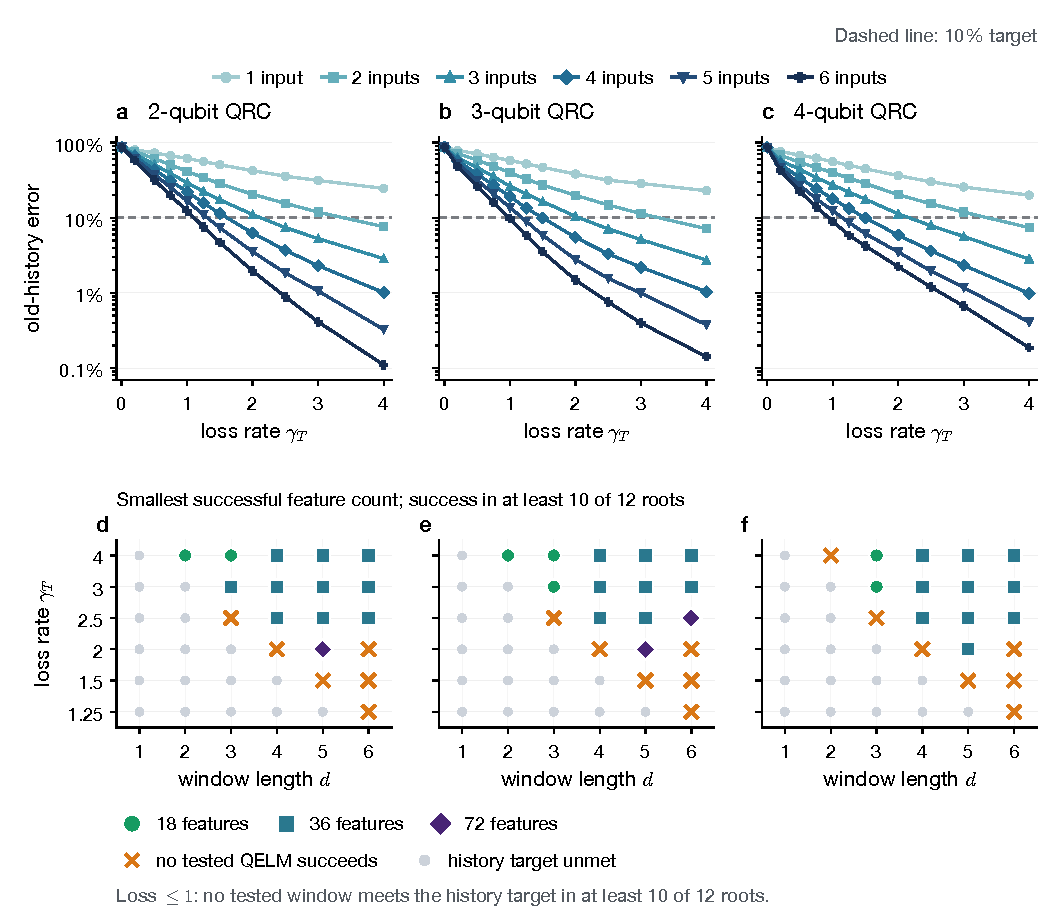
\includegraphics[width=\textwidth]{fig02_information_frontier.pdf}
 \caption{\textbf{When finite-window prediction becomes feasible.}
 For each displayed window, light gray means that output-relevant history
 remains outside that window at every tested feature budget.  Green, blue, and
 purple give the smallest successful budgets $B=18,36,72$, respectively, where
 success is the modal class across 12 independent roots at NRMSE tolerance
 $0.10$.  Orange is unresolved, and hatching marks root disagreement for at
 least one budget.  The map uses the frozen finite common-suffix panels drawn
 from the 33-symbol input alphabet.}
 \label{fig:information-frontier}
\end{figure*}

\subsection{Protected quantum memory cannot be replaced by a finite window}

A lasting obstruction needs one state quantity that an old input changes,
later inputs preserve, and the readout can observe.  A two-qubit singlet mode
has all three properties.  Its projector is visible through two-body Pauli
correlations, and symmetric channels leave it unchanged:
\begin{equation}
 \begin{aligned}
 P_-&=|\psi^-\rangle\!\langle\psi^-|
 =\frac{II-XX-YY-ZZ}{4},\\
 \Phi_{(u,0)}^\dagger(P_-)&=P_- .
 \end{aligned}
 \label{eq:protected-singlet}
\end{equation}
Here each time step uses the same time-homogeneous alphabet $a=(u,q)$.
The continuous value $u$ drives both qubits symmetrically; the flag $q$ applies
an addressable pulse to the first qubit.  After the old flagged input, the
allowed suffixes have arbitrary symmetric drives and $q=0$.  Exchange symmetry
and collective loss protect $P_-$, whereas the old local pulse changes its
population by
$\Delta p_-=\tfrac12\sin^2(0.5)=0.1149244235$.

Fix one infinite symmetric drive stream.  Two trajectories differ at the old
flagged input only and share every later input.  For a window of length $d$, we
evaluate after $d$ shared inputs.  The learner therefore sees identical data,
while the recurrent outputs retain the same gap.  For the two branches weighted
equally, let $R_{\rm pair}$ denote their mean squared prediction error.
Equation~\eqref{eq:window-law} and the appendix identity give
\begin{equation}
 \begin{aligned}
 E_d&\geq0.0574622 &&\text{for every finite }d,\\
 R_{\rm pair}&\geq0.0033019058 .
 \end{aligned}
 \label{eq:protected-floor}
\end{equation}
The same fixed recurrent process and fixed trajectory pair witness every
window.  The filter is therefore outside the fading-memory regime for the
declared output and symmetry-preserving suffix alphabet.

Numerical propagation over 12 independent couplings preserves the output gap
under collective loss to a maximum drift of $7.63\times10^{-16}$ through 80
suffix inputs.  Replacing collective by matched local loss reduces the median
gap to $1.57\times10^{-5}$ at step 80.  Small symmetry violations give a finite
certified persistence horizon; the short derivation is included below.

The information law itself is classical: any stateless window model faces the
same missing input.  The quantum physics lies in the mechanism that stores the
input, protects it with an open-system symmetry, and exposes it through Pauli
measurements.  Entanglement alone is not the obstruction.

\section{Numerical Experiments}
\label{sec:numerics}

The simulations distinguish three practical requirements for emulation.
The window must contain enough history, the fitted model must use that
information effectively, and the measurements must be sufficiently precise.
We examine these requirements in sequence.

\subsection{Models and Evaluation}

Our main experiments compare a fixed reset-QELM with two-, three-, and
four-qubit target QRCs. The targets have random $XX$ couplings, transverse
fields, input-dependent drives, and local loss $\gamma_T$, where $T$ denotes
the target QRC. Inputs are sampled uniformly from a 33-point alphabet on
$[0,1]$. Target outputs are single-site Pauli expectations and same-axis
two-site correlations.

The six-qubit reset-QELM encodes $d\leq6$ recent inputs, evolves under
independent random $XX$ couplings, and records Pauli features at nested times.
The original sweeps vary window length $d$, feature budget $B\in\{18,36,72\}$ counting
observable--checkpoint expectations, and circuit-shot budget per input $Q$.
These experiments evaluate a fixed feature architecture. The growing
universal family in Section~\ref{sec:criterion} establishes a separate
existence result.

Each independent realization block, called a root, fixes the target
parameters, input streams, and feature map. The confirmatory two- and
three-qubit cohort uses 12 roots. Dense maps use disjoint seeds, and a
prospectively specified four-qubit follow-up uses 12 new roots. A separate
prospective extension uses five-qubit targets, 12 new roots, and a ten-qubit
QELM with $d\in\{2,4,6,8,10\}$ and $B\in\{30,60,120\}$.
This extension increases both the available context and the emulator size.
Cohorts are analyzed separately.

Training, validation, test, and diagnostic streams are separate.
Standardization uses training data only, and validation selects the ridge
readout. Appendix~\ref{sec:methods} specifies the dynamics and fitting procedure.

To distinguish missing history from residual prediction error, we use a
held-out common-suffix panel. Different old histories are followed by
identical recent inputs. Mean squared variation around their mean output
measures the old-history contribution. The squared distance between that
mean and the emulator prediction measures the residual contribution.
These terms add exactly at the level of mean squared error
[Eq.~\eqref{eq:panel-decomposition}]. Residual emulator error can include
feature limitations, finite-data fitting, regularization, and finite-branch
estimation of the suffix mean. This sampled diagnostic does not directly
estimate the worst-case quantity $D_d$ or the spectral radius $r_{\rm vis}$.

Normalized root mean squared error (NRMSE) of $0.10$ corresponds to 10\%
of the target standard deviation. A setting meets the history or emulation
criterion when the corresponding error is at most $0.10$ in at least
10 of 12 roots. Confidence intervals use paired root-block bootstraps.

\begin{figure*}[t]
 \includegraphics[width=\textwidth]{fig04_long_context_n5.pdf}
 \caption{Five-qubit targets and longer context.
 Separate prospective cohort: 12 new roots and a fixed ten-qubit reset-QELM.
 \textbf{a,b} Common-suffix NRMSE versus window length at $\gamma_T=1$ and 4,
 comparing the history floor, $B=120$ QELM, and quadratic delay on logarithmic error axes.
 \textbf{c} Total QELM common-suffix NRMSE versus feature budget at fixed $d=10$
 on a linear error axis, using the same roots. Points show root medians; whiskers
 span the 10th--90th percentiles. Darker gray dashed lines mark 10\%.
 The larger emulator register is an additional resource, not a matched-size advantage.}
 \label{fig:long-context}
\end{figure*}

\subsection{History Requirements}

Longer windows and stronger local loss reduce the measured influence of
older inputs. Under weak loss, the missing past remains relevant throughout
the tested window range. Increasing loss shifts the minimum sufficient
window toward shorter contexts [Figure~\ref{fig:resource-diagnosis}(a)].

The dense maps cover 11 loss rates and windows from one to six, giving
198 size--loss--window settings across the two-, three-, and four-qubit
targets. Across these sizes, no tested window meets the history criterion
for $\gamma_T\leq1$. At $\gamma_T=4$, the minimum sufficient window is two
inputs. All rootwise local-loss decay fits have negative slopes in both
confirmatory sizes and in the independent four-qubit follow-up.

Longer context also improves the fitted QELM in the preregistered transition
settings. At $B=72$ and $\gamma_T\in\{2,4\}$, increasing $d$ from one to six
reduces held-out QELM NRMSE by a root median of $78.45\%$
(95\% CI $[76.64,80.80]\%$), with improvement in all 12 roots.
This measures the change in total emulator error, including both historical
and residual contributions.

The measured history-frontier pattern is robust to alternative success
thresholds. The primary $0.10$, 10-of-12 rule was preregistered.
A post hoc analysis uses tolerances $0.08$, $0.10$, and $0.12$, with 9, 10,
or 11 required roots. Individual crossing points change, but all 27 measured
history frontiers remain non-increasing with loss. Where no tested window
succeeds, the required context remains unresolved beyond the tested range.
These findings describe the tested systems and do not establish an
asymptotic size law.

The separate five-qubit extension shows what additional context can recover
[Figure~\ref{fig:long-context}(a,b)]. Increasing $d$ from two to ten reduces
history NRMSE by root medians of $93.55\%$ at $\gamma_T=1$ and $99.63\%$
at $\gamma_T=4$, with improvement in all 12 roots at each loss.
At $\gamma_T=1$, windows of six, eight, and ten inputs meet the history
criterion. At $\gamma_T=4$, every tested window meets it. The remaining
question is how effectively a fitted model can use this information.

\subsection{Feature Capacity and Classical Comparisons}

Sufficient history makes accurate emulation possible in principle, but
the tested feature model can still limit its accuracy. At $\gamma_T=4$,
a one-input window is history limited in every root even with $B=72$.
At $d=6$, history is sufficient, but the $B=18$ QELM usually fails while
replay succeeds. This is the operational representation-limit diagnosis
defined in Appendix~\ref{sec:methods}. With $B=36$, every root across the
two-, three-, and four-qubit targets reaches the tolerance.

Increasing feature capacity improves the residual error on this
history-sufficient setting. At $\gamma_T=4$ and $d=6$, increasing $B$ from
18 to 72 reduces common-suffix residual emulator NRMSE by a root median
of $67.26\%$ (95\% CI $[55.33,75.63]\%$).
The improvement occurs in all 12 roots in both confirmatory sizes
in the original cohort. All 24 confirmatory root-by-size
cases meet the emulation tolerance at $B=72$. The old-history term is unchanged.

A frozen follow-up extends the sweep to $B=144$ on 12 fresh roots per size
at $\gamma_T=4,d=6$, with fixed duration [Figure~\ref{fig:resource-diagnosis}(b)].
Exploratory $B=24,30$ reuse these data, retaining 18 final-time observables
and adding one or two per qubit at the midpoint with outcome-independent
Pauli-axis balance. Median error already declines before 36 features,
without isolating an approximation floor.

The five-qubit extension makes the distinction between history and fitted
accuracy particularly clear. At $\gamma_T=1$, no tested QELM budget meets
the total-error rule, even for the windows that meet the history criterion.
At $\gamma_T=4$, $B=60$ reaches the total-error tolerance in every root from
$d=4$ onward. At fixed $d=10$, most of the observed median-error reduction
occurs between 30 and 60 features, with little further decrease at 120
[Figure~\ref{fig:long-context}(c)]. These changes reflect the performance of
the fitted emulator, including feature approximation, estimation, and
regularization.

A longer window also need not improve fitted accuracy monotonically.
For each of the two-, three-, and four-qubit target sizes at $\gamma_T=2$
and $B=72$, $d=5$ meets the total-error rule while $d=6$ does not.
Window sufficiency and successful emulation must therefore be evaluated
separately.

Classical controls show how strongly the choice of model matters.
Linear delay, quadratic delay, and dimension-matched random-tanh models
use the same windows and data splits as the QELM. Quadratic delay is the
strongest classical control in all 24 fast-forgetting confirmatory cases
and outperforms the $B=72$ QELM in every root. In the five-qubit extension,
it also outperforms the $B=120$ QELM in 118 of 120 streaming root--condition
comparisons. These experiments demonstrate practical emulation limits
without establishing a quantum advantage.

\subsection{Measurement Budgets}

Additional features become useful only when measurements resolve them
accurately enough. We examine this requirement in a separate exploratory,
post-confirmatory study with 12 four-qubit targets at $\gamma_T=4$ and $d=6$,
where history is sufficient.

For each root, 16 repetitions independently sample training, validation,
and test features and repeat the complete fitting and selection procedure.
Validation selects both the ridge penalty and the feature budget.
Target outputs remain exact expectations, isolating the effect of finite
sampling in the emulator.

Median validation-selected test NRMSE falls from $0.231$ at 300 shots per
input to $0.0800$ at 19,200 shots [Figure~\ref{fig:resource-diagnosis}(c)].
The root median reduction is $65.20\%$ (95\% CI $[64.04,66.47]\%$),
with improvement in all 12 roots. Validation selects $B=36$ most often at
low shot budgets and $B=72$ at high budgets.

The useful feature budget therefore depends on the available measurement
budget. Once sufficient history is available, increasing feature capacity
and measurement precision together can improve practical emulation
\cite{hu2023sampling,ahmed2025finite}.

\FloatBarrier
\section*{Conclusions}
\label{sec:discussion}

For a bounded scalar observable output, a fixed input window is exact when its
common-suffix diameter is zero.  Growing windows approximate the output to
arbitrary accuracy when this diameter tends to zero.  Half of the diameter is
the smallest possible worst-case error of any stateless window predictor, so no
larger feature map can remove that floor.

Contractive QRC dynamics make the diameter decay exponentially, after which a
growing reset QELM can approximate the remaining continuous window function.
The two-qubit singlet construction gives the opposite case: an old input
changes a protected quantity that later symmetric dynamics preserve and Pauli
measurements reveal.  Its nonzero output gap survives every finite window.

The simulations turn the criterion into a practical diagnosis.  Increase the
window until the history floor is small, then increase the feature budget, and
finally supply enough shots to resolve those features.  The strongest classical
delay control outperforms the tested six-qubit QELM, so the result concerns
functional emulation and observable quantum memory rather than quantum
computational advantage.

\begin{figure*}[t]
 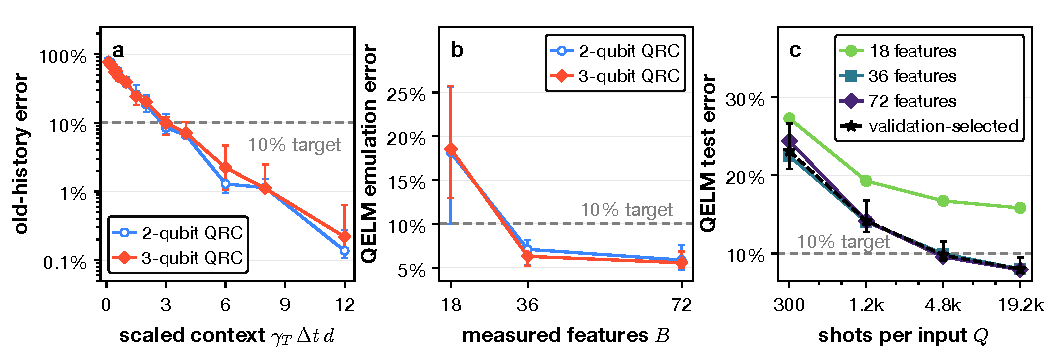
\includegraphics[width=\textwidth]{fig03_resource_diagnosis.pdf}
 \caption{\textbf{Three resources target three different limits.}
 \textbf{a} Longer windows reduce history NRMSE; curves are teacher-family
 medians and bands span the 10th--90th percentiles across roots.  \textbf{b}
 On the $\gamma_T=4,d=6$ slice, more measured features reduce total QELM
 NRMSE; faint curves are individual roots and heavy curves are teacher-family
 medians.  \textbf{c} More shots reduce total test NRMSE under finite
 measurement; curves are medians across 12 roots and the shaded selected-policy
 band spans their 10th--90th percentiles.  Dashed lines mark the NRMSE tolerance
 $0.10$.  \textbf{c} is a post-confirmatory four-qubit study with 16
 complete fit-and-selection replicates per root.}
 \label{fig:resource-diagnosis}
\end{figure*}

\appendix
\section{Short derivations}

\subsection{The window law}

For a fixed suffix $s$, write $y_-(s)$ and $y_+(s)$ for the infimum and
supremum of its compatible outputs.  Any suffix predictor returns one number
on this set, so values arbitrarily close to the two endpoints force an error
of at least
$[y_+(s)-y_-(s)]/2$.  The midpoint
$[y_+(s)+y_-(s)]/2$ reaches this bound.  Taking the supremum over suffixes proves
Eq.~\eqref{eq:window-law}.  The same lower bound holds for a randomized output
$A$, because
$|y_+-y_-|\leq\mathbb E|y_+-A|+\mathbb E|y_--A|$.  For a balanced pair,
\begin{equation}
 \frac12\sum_{b=0}^1\mathbb E(y_b-A)^2
 =\frac{(y_1-y_0)^2}{4}
  +\mathbb E\!\left[A-\frac{y_0+y_1}{2}\right]^2 .
\end{equation}

\subsection{The protected singlet}

If every allowed suffix channel satisfies $\Phi_a^\dagger(P_-)=P_-$, then any
composition of those channels does too.  The singlet population difference is
therefore unchanged by every finite allowed suffix.  The old pulse loads it
because
\begin{equation}
 \begin{aligned}
 R_x^{(1)}(\theta)|00\rangle
 &=\cos(\theta/2)|00\rangle-i\sin(\theta/2)|10\rangle,\\
 |\langle\psi^-|10\rangle|^2&=\frac12 .
 \end{aligned}
\end{equation}
This gives $\Delta p_-=\tfrac12\sin^2(\theta/2)$, while
$P_-=(II-XX-YY-ZZ)/4$ makes the population measurable from the stated Pauli
outputs.

For imperfect protection, let
$\varepsilon_{\rm prot}=\sup_a\|\Phi_a^\dagger(P_-)-P_-\|_\infty$.  Each
allowed step can reduce the branch gap by at most
$2\varepsilon_{\rm prot}$, because the trace norm of the difference between
two states is at most two.  Summing over $d$ steps gives the readable
finite-horizon bound
\begin{equation}
 |\Delta p_d|\geq
 \max\{0,|\Delta p_0|-2d\varepsilon_{\rm prot}\}.
\end{equation}

\subsection{The reset-QELM bound}

Let $\widetilde\rho_t^{(d)}$ be the state obtained by replaying the final $d$
channels from one fixed reset state.  Repeated contraction gives
\begin{equation}
 D_{\rm tr}(\rho_t,\widetilde\rho_t^{(d)})\leq\eta^d,
 \qquad
 |Y_t-\operatorname{Tr}(O\widetilde\rho_t^{(d)})|\leq2M\eta^d .
\end{equation}

For each window coordinate $x_i$, prepare $r$ qubits in
$\sqrt{1-x_i}|0\rangle+\sqrt{x_i}|1\rangle$ and record the Hamming weight
$K_i$.  Then $K_i\sim\operatorname{Binomial}(r,x_i)$.  If $g_d$ is the replay
output, a linear readout with coefficients $g_d(\boldsymbol k/r)$ returns the
Bernstein polynomial $\mathbb E[g_d(\boldsymbol K/r)]$.  Input Lipschitzness
and contraction give
\begin{equation}
 |g_d(\boldsymbol x)-g_d(\boldsymbol y)|
 \leq2ML_u\sum_{i=1}^d\eta^{d-i}|x_i-y_i|.
\end{equation}
Since
$\mathbb E|K_i/r-x_i|\leq1/(2\sqrt r)$, the Bernstein error is at most
$ML_u(1-\eta^d)/[(1-\eta)\sqrt r]$.  Finally, each circuit shot produces a
score in $[-M,M]$.  Hoeffding's inequality bounds the error of the mean of $Q$
scores by
$M\sqrt{2\log(2/\alpha)/Q}$ with probability at least $1-\alpha$.  Adding the
three errors proves Eq.~\eqref{eq:qrc-qelm-bound}.

For a general continuous fading-memory filter, choose a finite window whose
truncation error is below half the target tolerance.  The remaining map is a
continuous function on a compact finite-dimensional domain, so Bernstein
approximation supplies a finite reset QELM for the other half.  This proves the
stated general corollary without assuming exponential contraction.

\section{Numerical methods and reproducibility}
\label{sec:methods}

\subsection{Protected-memory construction}

The protected-memory QRC starts in $|00\rangle$ with
$H(u)=JX_1X_2+0.37(Z_1+Z_2)+0.64u(X_1+X_2)$ and collective jump
$L_c=\sqrt{0.8}(\sigma_1^-+\sigma_2^-)$, where
$\sigma_i^-=|0\rangle\langle1|_i$ is the lowering operator on qubit $i$.
Steps last $\Delta t=0.2$. An old flag applies $I$ or $R_x^{(1)}(1)$
(a one-radian rotation), followed by 80 unpulsed inputs $u\in[0,1]$.
Twelve roots independently sample $J\in[-1,1]$ and suffixes. Checks verify
conserved singlet population, its analytic pulse value, and zero population
under symmetric preparation. With matched local amplitude damping,
the median absolute 80-step gap is $1.569\times10^{-5}$.
Relative collective-jump asymmetries $0.02$, $0.05$, $0.10$, and $0.20$
produce nonzero initial singlet decay, not necessarily rapid erasure.

\subsection{Target QRCs and reset-QELM emulator}

Target QRCs (subscript $T$) have $N_T\in\{2,3,4\}$ qubits and local-loss
rate $\gamma_T$. Each fixed scalar input $a$ drives
\begin{align}
 H_T(a)&=\sum_{i<j}J_{ij}X_iX_j+0.5\sum_i Z_i+a\sum_iX_i,\nonumber\\
 \dot\rho&=-i[H_T(a),\rho]+\gamma_T\sum_i\mathcal D[\sigma_i^-]\rho,
 \label{eq:target-qrc-model}
\end{align}
where $\dot\rho=d\rho/d\tau$ uses continuous physical time $\tau$, while
$t$ indexes discrete inputs. The dissipator is
$\mathcal D[L]\rho=L\rho L^\dagger-\tfrac12\{L^\dagger L,\rho\}$;
$\dagger$, $[\cdot,\cdot]$, and $\{\cdot,\cdot\}$ denote Hermitian adjoint,
commutator, and anticommutator. Couplings are uniform on $[-1,1]$,
$\Delta t=0.5$, and inputs use a uniform 33-point alphabet on $[0,1]$.
All single-site Pauli expectations and same-axis two-site products give
9, 18, and 30 outputs for $N_T=2,3,4$.

The fixed six-qubit QELM resets each prediction and encodes the newest
$d\leq6$ inputs separately as
$\sqrt{1-a}|0\rangle+\sqrt a|1\rangle$, leaving unused qubits in $|0\rangle$.
An independent random $XX$ Hamiltonian with uniform $[-1,1]$ couplings
and transverse field $0.5$ evolves each reset product state for $\tau=0.5$
without dissipation. Single-site $X,Y,Z$ expectations at one, two, or four
nested checkpoints give $B\in\{18,36,72\}$ observable--checkpoint features.

Training alone standardizes features. Validation selects affine ridge
penalty $\lambda$ from
$\{0,10^{-10},10^{-8},10^{-6},10^{-4},10^{-2},1,10^2,10^4,10^6,\infty\}$;
the readout is then refitted on training and validation. Finite penalties
use economy singular-value decomposition with relative resolved-subspace
cutoff $10^{-6}$; $\lambda=\infty$ denotes intercept-only prediction.

\subsection{Cohorts, panels, and decision rules}

The confirmatory cohort uses $N_T\in\{2,3\}$,
$\gamma_T\in\{0,0.2,0.5,1,2,4\}$, and $d\in\{1,2,4,6\}$.
The dense map adds $d=3,5$ and rates $0.75,1.25,1.5,2.5,3$ with
12 roots and 108 seeds disjoint from the original experiment.
After map inspection, the four-qubit follow-up was prospectively frozen:
12 new roots, 96 disjoint seeds, and unchanged rates, windows, emulator,
budgets, sample sizes, and success rule. Registered checks test negative
history decay, a non-increasing minimum-window frontier, and the
$\gamma_T=4,d=6,B=72$ anchor. Size cohorts are never pooled.

Each root has independent train, validation, test, and suffix streams.
Streaming splits start in $|0\cdots0\rangle$: 128 washout steps precede
480 training, 160 validation, or 320 test rows. Panels contain 32 length-six
suffixes, each following four independently burned-in prefixes; shorter
windows are nested tails. Newest suffix symbols are sampled without replacement
from the alphabet; older coordinates are independent. Couplings, streams,
and feature seeds are fixed within roots; seed namespaces are disjoint across
roots and cohorts. The held-out panel diagnostic does not directly estimate
$D_d$ or $r_{\rm vis}$.

The preregistered $0.10$ tolerance is 10\% of the target standard deviation;
history sufficiency requires at least 10 of 12 roots below or at it.
Under fair nonzero signs, at least 10 of 12 agreeing gives one-sided
probability $0.0193$. Independent units are roots, not rows, observables,
suffixes, or shot replicates; confidence intervals use 20,000 paired
root-block bootstraps.

After excluding variances below $10^{-8}$, the decision order checks
history-floor failure, total-QELM success, then replay success.
Representation limited operationally means history passes, the fitted QELM
fails, and replay succeeds; it does not isolate the best approximation using
QELM features.

Linear delay, quadratic delay, dimension-matched random-tanh, intercept-only,
and reset--replay share windows and splits. Replay applies the target's final
$d$ channels to a fixed state: retrained replay refits weights; compiled
replay retains a trained affine readout. Each cell selects the best of the
three nonconstant classical controls. The $0.10$, 10-of-12 frontier predates
dense-cohort inspection; post hoc sensitivity checks reuse the simulations
at tolerances $0.08$, $0.10$, $0.12$ and 9, 10, or 11 required roots.

\subsection{Finite-shot and long-context extensions}

The finite-shot study uses 12 four-qubit local-loss targets,
$\gamma_T=4$, $d=6$, and $Q\in\{300,1200,4800,19200\}$ shots per input.
Snapshots and global-Pauli settings receive equal integer shares;
joint multinomial bit-string draws supply compatible single-site expectations.
Each of 16 replicates resamples train, validation, and test features
independently and repeats fitting. Validation selects $\lambda$ for each $B$,
then $B$, without test targets. Target outputs remain exact.

The separate prospective long-context cohort uses 12 new roots,
five-qubit local-loss targets with 45 outputs, $\gamma_T\in\{1,4\}$,
and $d\in\{2,4,6,8,10\}$. A fixed ten-qubit QELM encodes one input per
qubit; nested checkpoints give $B\in\{30,60,120\}$. Panels use 32
length-ten suffixes with four prefixes each; other settings are inherited.
Freezing follows two duplicate development runs and dense-backend checks.
All cells remain; paired history contrasts use 10,000 root-block
bootstrap draws, and the QELM--quadratic comparison fixes $B=120$ before
test evaluation. Cross-cohort changes include register size, not context alone.

All evidence is simulated, excluding hardware, gate,
state-preparation-and-measurement, drift, and measurement-backaction errors.
The stated theorem assumptions do not make the tested feature map universal
or supply a sample-efficient training algorithm.


\bibliography{references}

\end{document}
